\documentclass{article}

\usepackage{amsmath}
\usepackage[utf8]{inputenc}
\usepackage[italian]{babel}
\usepackage{hyperref}
\usepackage{graphicx}
\usepackage{minted}
\usepackage{tikz}
\usepackage{tabularx}
\usepackage{framed}
\usepackage{geometry}
\usepackage{parskip}
\usepackage{tabularx}
\usepackage{enumitem}
\usepackage{float}
\usepackage{color,colortbl}
\usepackage{tocloft}
\usepackage{afterpage}
\usepackage{xparse}
\usepackage[stretch=10,shrink=10]{microtype}

% Set path for pictures
\graphicspath{ {./images/} }

% Do not indent on new paragraphe
% \setlength{\parindent}{0pt}

% Newline after paragraphe title
\makeatletter
\renewcommand\paragraph{\@startsection{paragraph}{4}{\z@}%
   {-3.25ex\@plus-1ex \@minus-.2ex}%
   {1.5ex \@plus.2ex}%
   {\normalfont\normalsize\bfseries}}
\makeatother


\newcommand{\myparskip}{\setlength{\parskip}{.8em}}
\newcommand{\noparskip}{\setlength{\parskip}{0pt}}
\definecolor{link}{rgb}{0,0,.6}


\def\ifempty#1{\def\temp{#1} \ifx\temp\empty}
\newcommand{\code}[1]{\texttt{#1}}

% Wrapper for new image.
% [#1]: scale factor
% {#2}: file path
% {#3}: caption
% {#4}: label (ID for links etcs)
\NewDocumentCommand{\image}{ O{} m m m }{%
  \begin{figure}[ht]
    \centering
    \caption{#3}
    \vspace{2pt}
    \includegraphics[width=#1\linewidth]{#2}%
    \label{fig:#4}
  \end{figure}
  \afterpage{\clearpage}
}
\NewDocumentEnvironment{custenum}{ O{} }{%
  \begin{enumerate}[topsep=2pt,label=\arabic*.#1]
    \setlength{\itemsep}{2pt}
    \setlength{\parskip}{0pt}
    \setlength{\parsep}{0pt}
}{%
  \end{enumerate}
}
\NewDocumentEnvironment{custlist}{ O{} }{%
  \begin{itemize}[topsep=2pt#1]
    \setlength{\itemsep}{2pt}
    \setlength{\parskip}{0pt}
    \setlength{\parsep}{0pt}
}{%
  \end{itemize}
}
\NewDocumentEnvironment{custdesc}{ O{} }{%
  \begin{description}[topsep=2pt#1]
    \setlength{\itemsep}{2pt}
    \setlength{\parskip}{0pt}
    \setlength{\parsep}{0pt}
}{%
  \end{description}
}
\NewDocumentEnvironment{specifica}{ m m m }{%
  \begin{framed}
    \noparskip{}
    \textbf{Attori}: #1\\
    \ifempty{#2} \empty\else \textbf{Precondizioni}: #2 \fi
    \textbf{Passi}:
    \begin{custenum}
}{%
    \end{custenum}
    \ifempty{#3} \empty\else \textbf{Postcondizioni}: #3 \fi
  \end{framed}
}


\hypersetup{%
    pdfborder = {0 0 0}
}

\title{Documentazione Progetto Ingegneria del Software}
\author{XXXXXXXX Luca, XXXXXXXX Laura\\
        VRXXXXXX, VRXXXXXX}
\date{20/05/2021}

\begin{document}
\maketitle

\newpage

\tableofcontents

\newpage

\section{Note introduttive}

Il sistema proposto, a cui è stato assegnato il nome "vaxplan", è un sistema software ad uso di una ASL (Azienda Sanitaria Locale) generica. Il sistema è pensato per essere usato in primis dal personale, che è a carico di indire o modificare campagne vaccinali, e dai cittadini, che utilizzeranno il software - presumibilmente su un totem pubblicamente disponibile o sulla propria macchina personale - per prenotare una data di vaccinazione.

\section{Requisiti}

\subsection{Requisiti non funzionali}

La ASL destinataria di questo sistema ha bisogno di essere in grado di avere un alto livello di controllo sulle campagne vaccinali. Un operatore ASL deve, infatti, essere in grado di poter indire una campagna vaccinale qualsiasi, specificando opportunamente il periodo di date entro le quali questa campagna vaccinale è valida, il range di ore in cui i centri vaccinali saranno aperti, oltre che il numero di dosi di vaccino disponibili, gli ambulatori in cui sarà possibile usufruire di tale campagna, ed eventualmente quali categorie di pazienti hanno accesso alla vaccinazione.

Diverse campagne vaccinali possono infatti essere ristrette ad una certa fascia della popolazione sia per ragioni tecniche che per ragioni politiche: da un lato possono esistere delle controindicazioni a somministrare un dato vaccino su persone che sono in una determinata condizione, dall'altro situazioni di scarsità di dosi di un determinato vaccino possono costringere l'ASL ad effettuare delle scelte e di indire campagne vaccinali solo per determinate fasce della popolazione che sono particolarmente a rischio da una data malattia.

La ASL deve inoltre essere in grado, in qualsiasi momento, di cambiare ogni parametro della campagna vaccinale. Per esempio, dal momento che le dosi che vengono riservate per una data prenotazione da parte di un cittadino vengono automaticamente rimosse dal conteggio delle dosi di vaccino disponibili per una determinata campagna vaccinale, è dunque necessario consentire di registrare eventuali dosi aggiuntive allocate in un secondo momento dopo aver indetto la campagna vaccinale. Questo è particolarmente importante per le campagne vaccinali contro il COVID-19, poiché è stato osservato che la disponibilità di dosi di vaccino non è sempre sufficiente a soddisfare adeguatamente l'elevatissima domanda, situazione che costringe a comprare in continuazione nuovi lotti di vaccini contro il COVID-19.

È inoltre necessario prevenire false prenotazioni mantenendo un database di pazienti residenti nella regione in cui la ASL in questione opera.

\newpage

\section{Scenari d'uso}

\begin{center}
    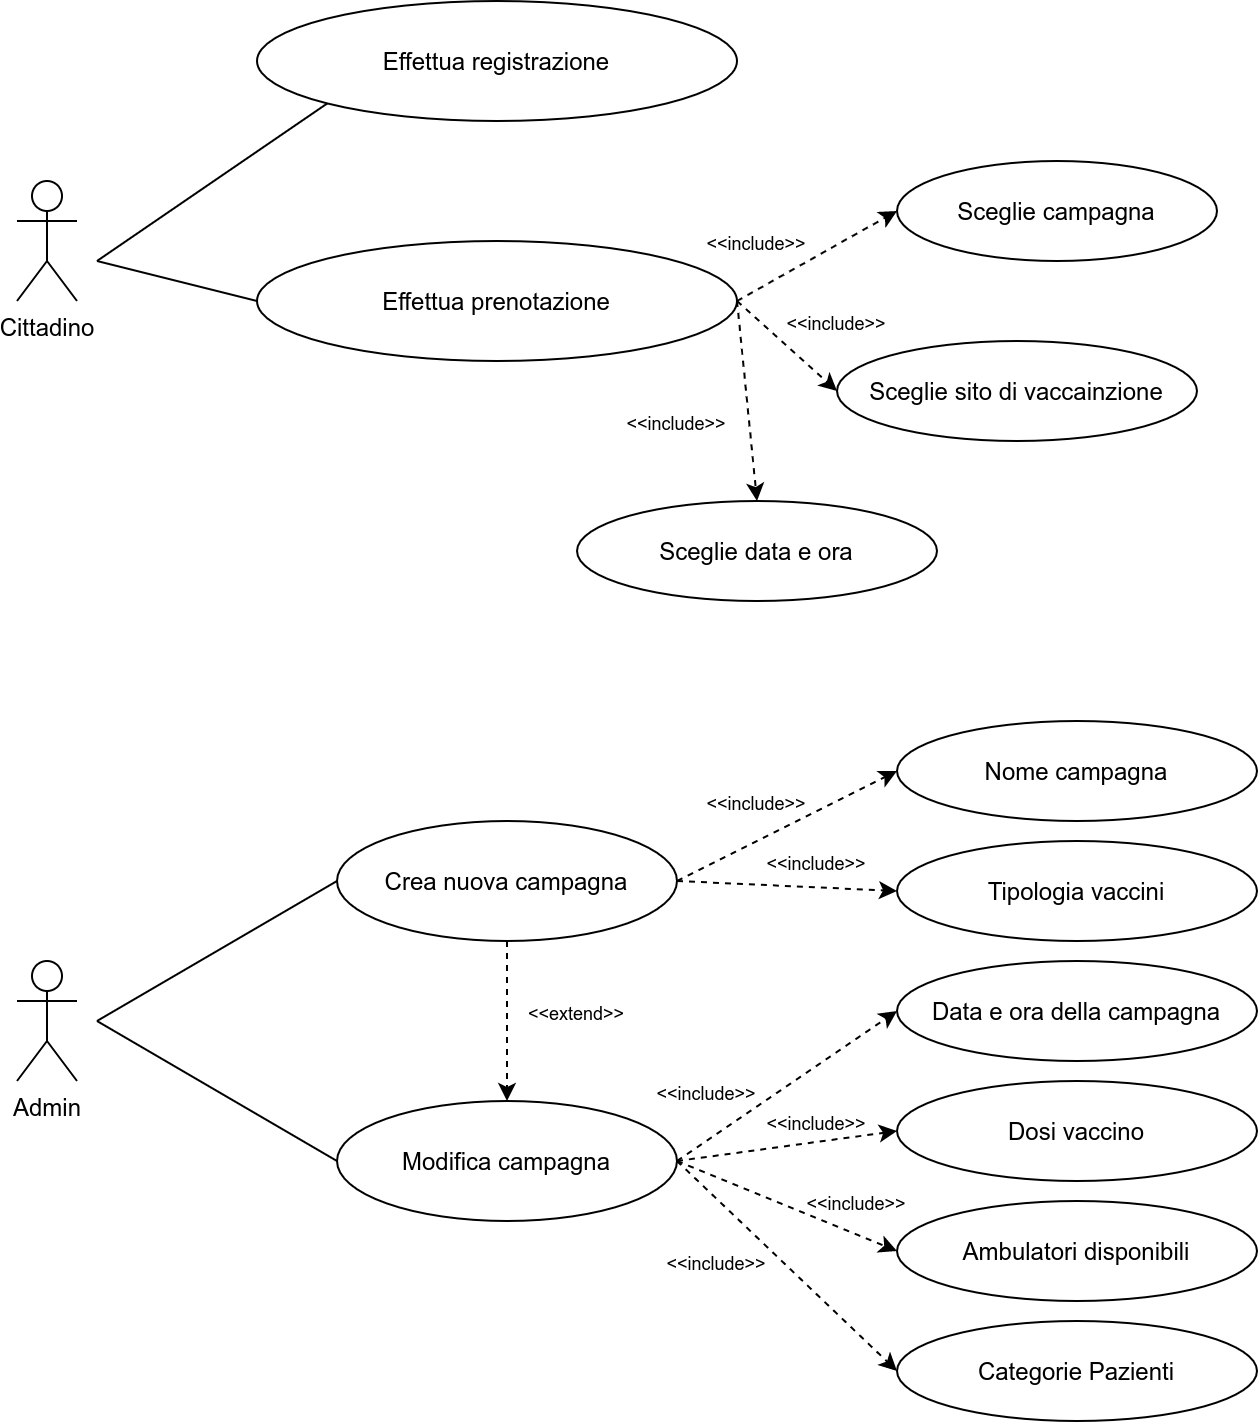
\includegraphics[scale = 0.25]{usecase_diagram.png}
\end{center}

\subsection{Creazione campagna vaccinale da parte del personale ASL}

Il sistema consente di gestire un elenco di campagne vaccinali. È a carico del personale ASL creare le campagne vaccinali a cui i cittadini potranno, in un secondo momento, aderire. Il personale ASL ha controllo completo sulla campagna.

Il sistema non è inizializzato con nessuna campagna vaccinale al primo avvio, quindi è necessario che questo caso d'uso venga eseguito per primo.

\newpage

\begin{framed}
    \noparskip{}
    \textbf{Attori}: Addetto personale ASL\\
    \textbf{Precondizioni}: L'addetto deve trovarsi sul pannello di amministrazione
    \begin{enumerate}
        \item L'addetto clicca su "Nuova campagna"
        \item L'addetto riempie i campi con le informazioni necessarie, interagendo opportunamente  con i vari campi di testo e bottoni
            \begin{itemize}
                \item seleziona il nome della campagna
                \item seleziona il tipo di vaccino da somministrare nella campagna
                \item specifica il numero di dosi disponibili
                \item specifica gli ambulatori in cui la campagna è disponibile
                \item specifica le categorie di pazienti che possono beneficiare della campagna
                \item specifica la data di inizio e di fine della campagna
                \item specifica l'ora di inizio e di fine della campagna
            \end{itemize}
        \item L'addetto clicca sul pulsante "Conferma" in basso a destra sulla finestra
    \end{enumerate}
    \textbf{Postcondizioni}: La campagna viene creata secondo le preferenze dettate dall'addetto e  aggiunta alla lista delle campagne vaccinali
\end{framed}

\begin{center}
    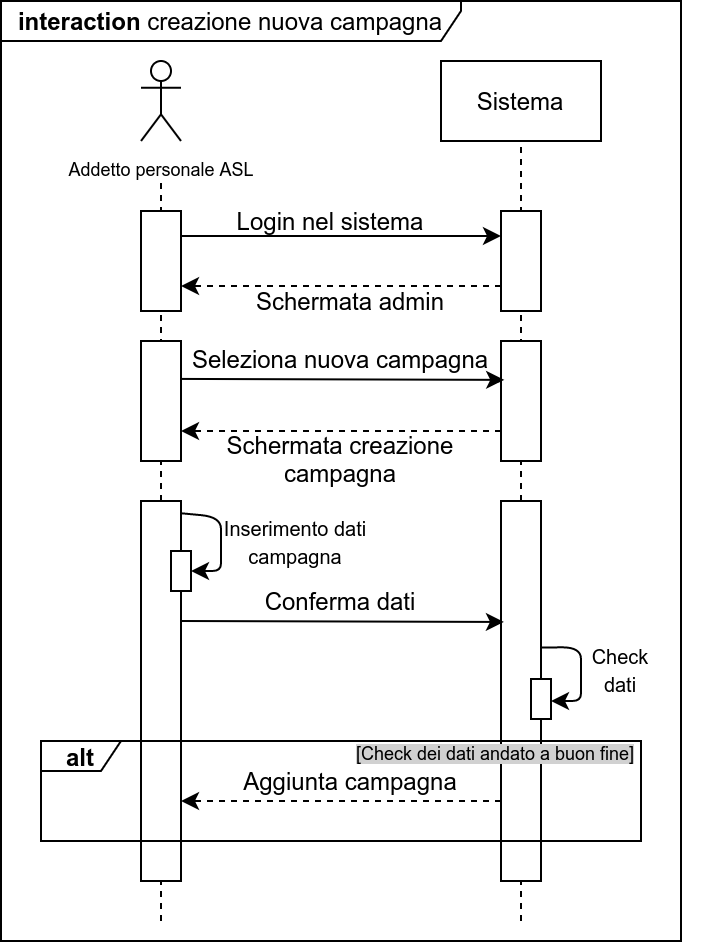
\includegraphics[scale=0.25]{sequence_diagram_usecase_new_campaign.png}
\end{center}

Si noti che il nome della campagna può essere arbitrario e non deve necessariamente corrispondere con il vaccino che verrà somministrato. Quest'ultimo non deve essere immesso da tastiera, ma deve essere scelto da una lista di vaccini già definita da un ComboBox.

Per quanto riguarda invece la selezione degli ambulatori disponibili e delle categorie di pazienti a cui il vaccino è rivolto, nel momento in cui l'addetto clicca uno dei bottoni predisposti per questo, si apre in una nuova finestra una vista che consiste di due liste affiancate e di due pulsanti che consentono di spostare elementi tra di loro. La lista sulla sinistra corrisponde alla lista degli elementi disponibili, mentre quella sulla destra corrisponde agli elementi selezionati.

\newpage

\subsection{Modifica campagna vaccinale da parte del personale ASL}

\begin{framed}
    \noparskip{}
    \textbf{Attori}: Addetto personale ASL\\
    \textbf{Precondizioni}: L'addetto deve trovarsi sul pannello di amministrazione
    \begin{enumerate}
        \item L'addetto clicca sul selettore delle campagne vaccineli attive denominato "Seleziona campagna vaccinale..."
        \item L'addetto clicca sul pulsante OK
        \item L'addetto clicca sulla scheda che corrisponde a ciò che vuole modificare ed effettua la modifica opportuna
            \begin{itemize}
                \item numero di dosi
                \item intervallo di date e ore associate alla campagna
                \item ambulatori disponibili per la campagna
                \item categorie di pazienti
            \end{itemize}
        \item L'addetto clicca sul pulsante "Conferma" in basso a destra sulla finestra
    \end{enumerate}
    \textbf{Postcondizioni}: La campagna viene modificata secondo le preferenze dettate dall'addetto
\end{framed}

La modifica della campagna è, dal punto di vista dell'utente, completamente analoga all'aggiunta, con la differenza che le view associate ai parametri della campagna da modificare sono organizzati in schede nella singola finestra.

\begin{center}
    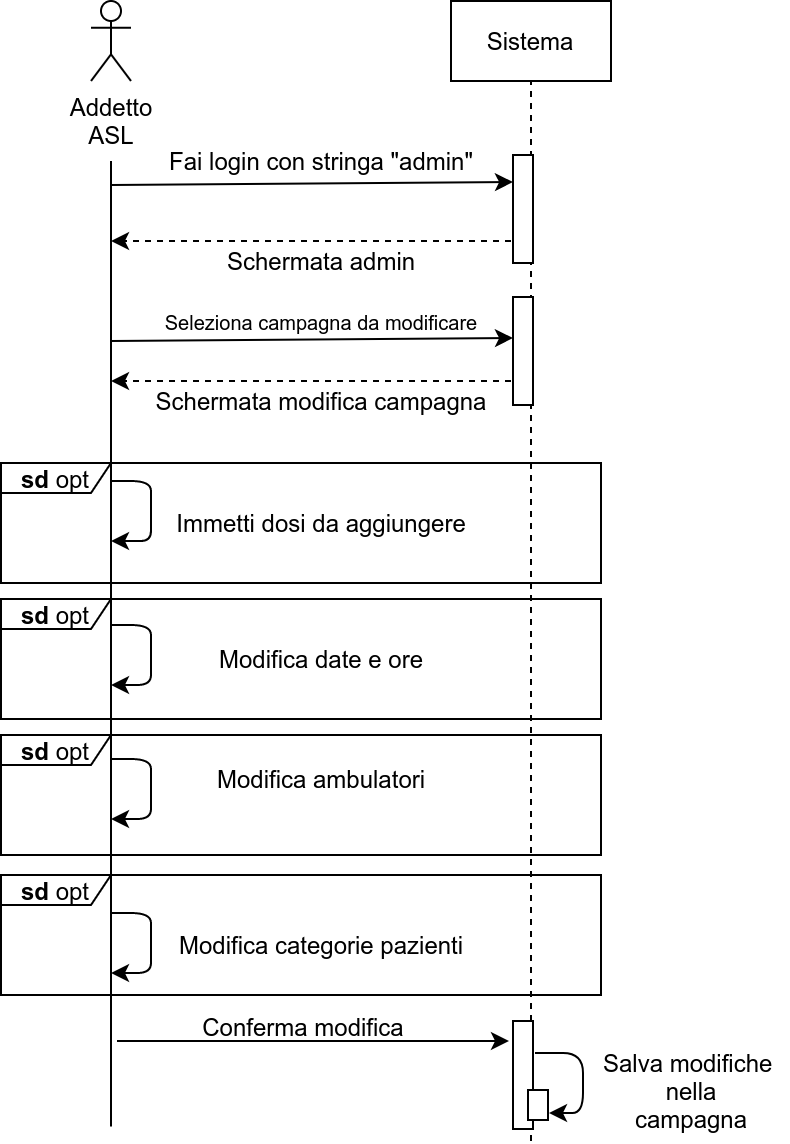
\includegraphics[scale=0.25]{sequence_diagram_usecase_edit_campaign.png}
\end{center}

\newpage

\subsection{Prenotazione campagna vaccinale da parte di un cittadino}

In questa fase, vi sono tre scenari alternativi:

\begin{itemize}
    \item L'utente è un paziente registrato ed è presente nel database della regione
    \item L'utente non è registrato, ma è presente nel database della regione
    \item L'utente non è registrato e non è presente nel database della regione
\end{itemize}

\begin{framed}
    \noparskip{}
    \textbf{Attori}: Cittadino\\
    \textbf{Precondizioni}: Essere già registrato al sistema
    \begin{enumerate}
        \item L'utente inserisce il proprio codice fiscale e tenta il login
        \item L'utente seleziona la campagna vaccinale 
        \item L'utente seleziona una sede di vaccinazione
        \item L'utente seleziona la data che preferisce
        \item L'utente seleziona l'ora che prefereisce tra quelle mostrate
        \item L'utente visualizza una schermata di conferma della prenotazione, riassuntiva di tutti i dettagli rilevanti
            \begin{itemize}
                \item nome e cognome paziente
                \item nome della campagna
                \item data della prenotazione
                \item intervallo di tempo della prenotazione
            \end{itemize}
    \end{enumerate}
    \textbf{Postcondizioni}: L'utente ha completato la prenotazione
\end{framed}

\begin{framed}
    \noparskip{}
    \textbf{Attori}: Cittadino\\
    \textbf{Precondizioni}: Essere nel database dei cittadini della regione ma non essere registrato
    \begin{enumerate}
        \item L'utente inserisce il proprio codice fiscale e tenta il login
        \item L'utente viene portato sullo schermo di registrazione, dove inserisce i suoi dati anagrafici
            \begin{itemize}
                \item nome
                \item cognome
                \item data di nascita
                \item luogo di nascita
                \item codice fiscale
                \item sesso
            \end{itemize}
        \item L'utente visualizza una lista di categorie di pazienti a cui appartiene
        \item L'utente seleziona, tra le campagne disponibili, quella a cui desidera aderire
        \item L'utente seleziona una sede di vaccinazione tra quelle disponibili
        \item L'utente seleziona la data che preferisce tra quelle mostrate
        \item L'utente seleziona l'ora che prefereisce tra quelle mostrate, in range di 10 minuti
        \item L'utente visualizza una schermata di conferma della prenotazione riassuntiva di
            \begin{itemize}
                \item nome e cognome paziente
                \item nome della campagna
                \item data della prenotazione
                \item intervallo di tempo della prenotazione
            \end{itemize}
    \end{enumerate}
    \textbf{Postcondizioni}: L'utente ha completato la prenotazione
\end{framed}

\begin{framed}
    \noparskip{}
    \textbf{Attori}: Cittadino\\
    \textbf{Precondizioni}: Non essere né registrato, né essere presente nel database dei cittadini della ragione
    \begin{enumerate}
        \item L'utente inserisce il proprio codice fiscale e tenta il login
        \item L'utente viene portato sullo schermo di registrazione, dove inserisce i suoi dati anagrafici
            \begin{itemize}
                \item nome
                \item cognome
                \item data di nascita
                \item luogo di nascita
                \item codice fiscale
                \item sesso
            \end{itemize}
        \item Quando l'utente prova a confermare la registrazione, non gli viene permesso di procedere oltre
    \end{enumerate}
    \textbf{Postcondizioni}: L'utente non è in grado di usufruire del sistema
\end{framed}

Questo caso d'uso viene gestito così in quanto si assume che la ASL in questione operi su scala unicamente regionale e che non sia prevista la prenotazione di vaccinazioni per cittadini non residenti nella regione in cui la ASL opera tramite la piattaforma online.

\begin{center}
    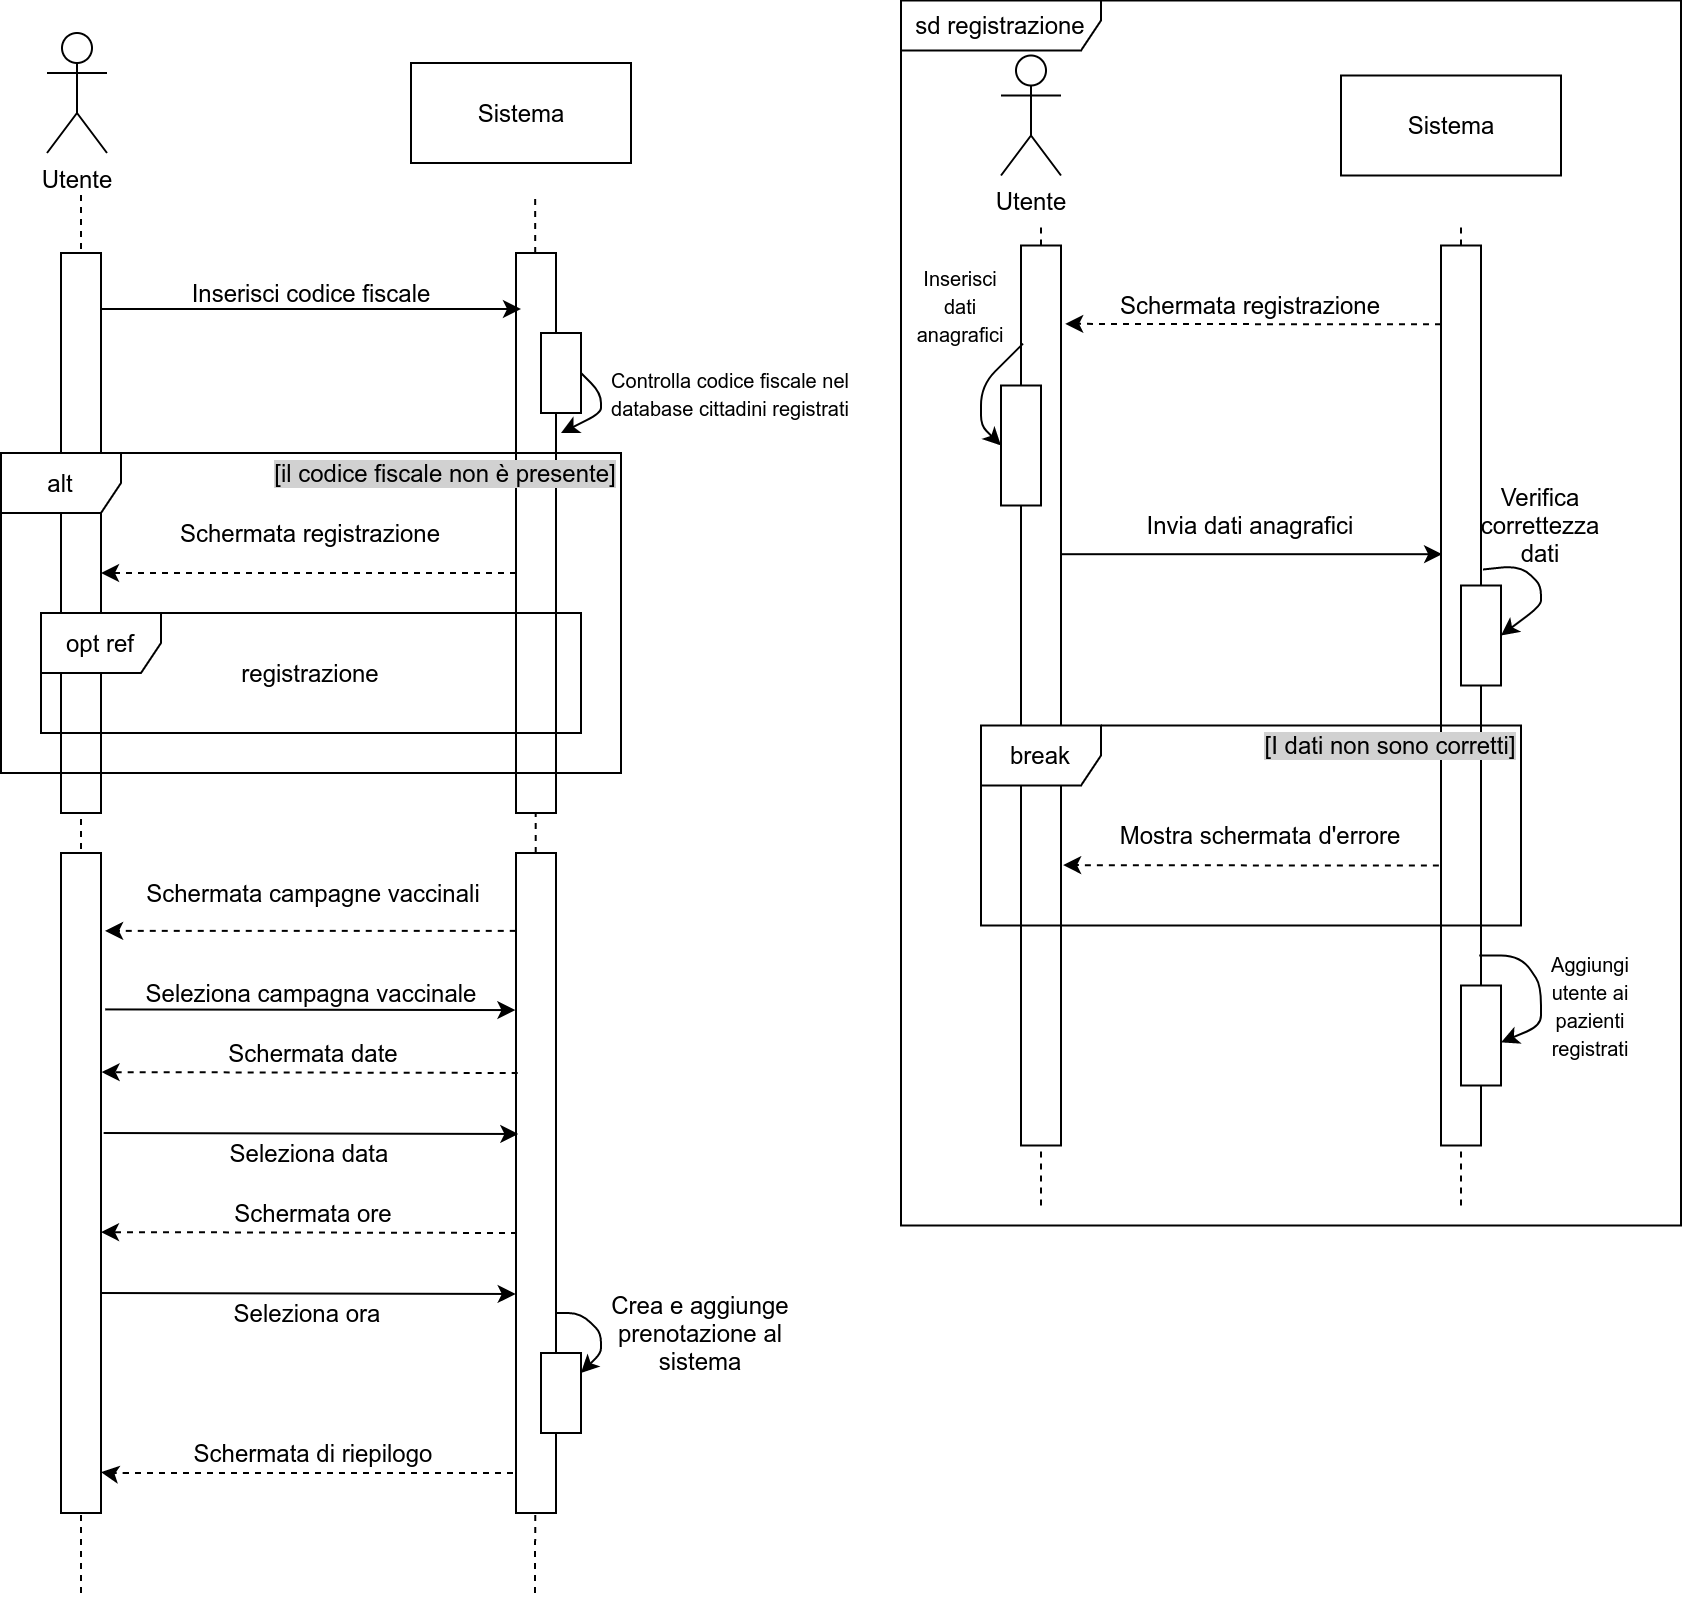
\includegraphics[scale=0.25]{sequence_diagram_usecase_book_campaign.png}
\end{center}

\subsection{Diagrammi di attività}

Si noti che questi activity diagram sono stati realizzati senza considerare la possibilità di ripetere più volte o annullare prima del compimento le attività qui rappresentate. Lavorare senza questa assunzione avrebbe portato a dei diagrammi decisamente meno semplici e comprensibili, cosa che sarebbe risultata controproducente rispetto al fine che un activity diagram tradizionalmente ha.

\begin{center}
    \begin{figure}
        \centering
        \caption{Diagramma di attività del cittadino}
        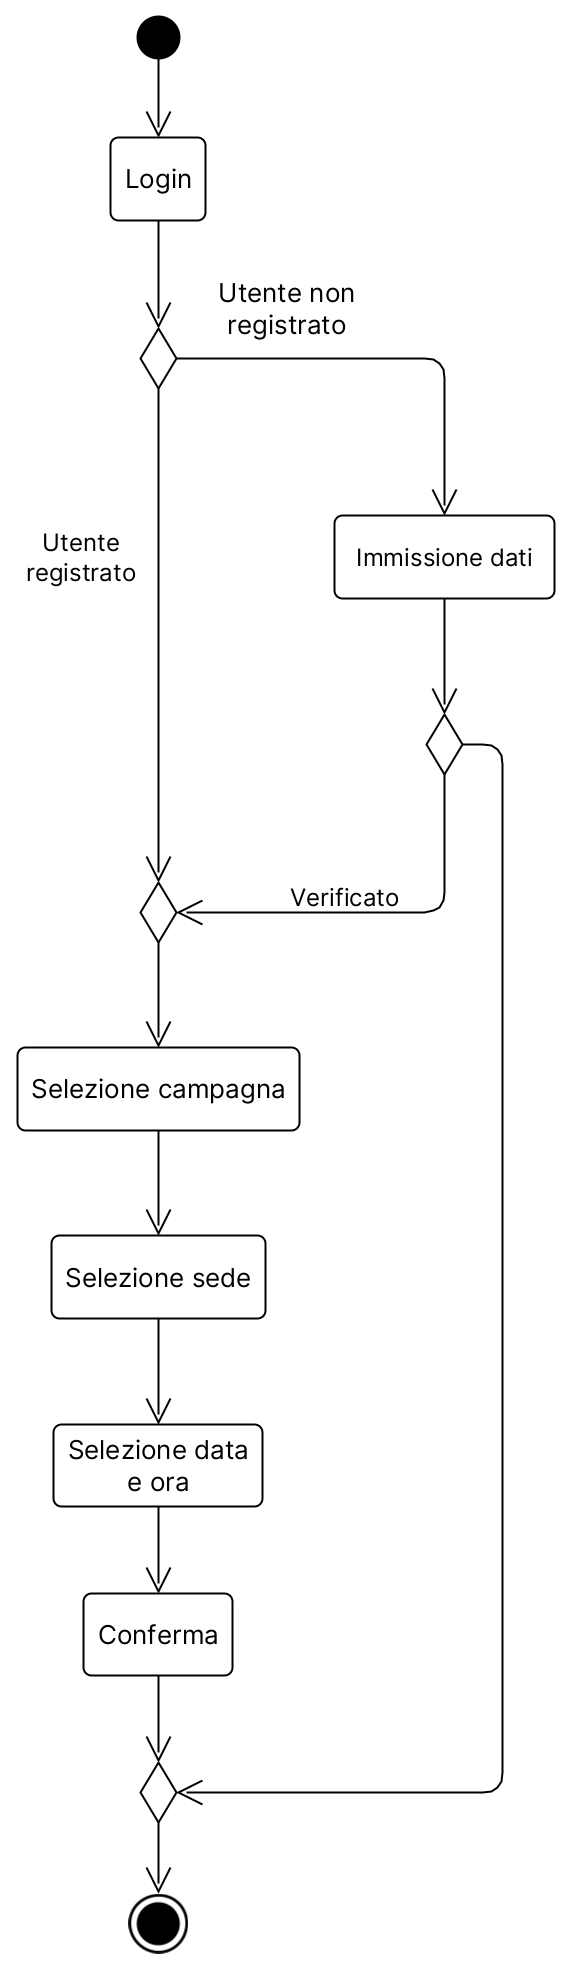
\includegraphics[scale=0.25]{ad_citizen_yed.png}
    \end{figure}
\end{center}

\begin{center}
    \begin{figure}
        \centering
        \caption{Diagramma di attività dell'addetto ASL}
        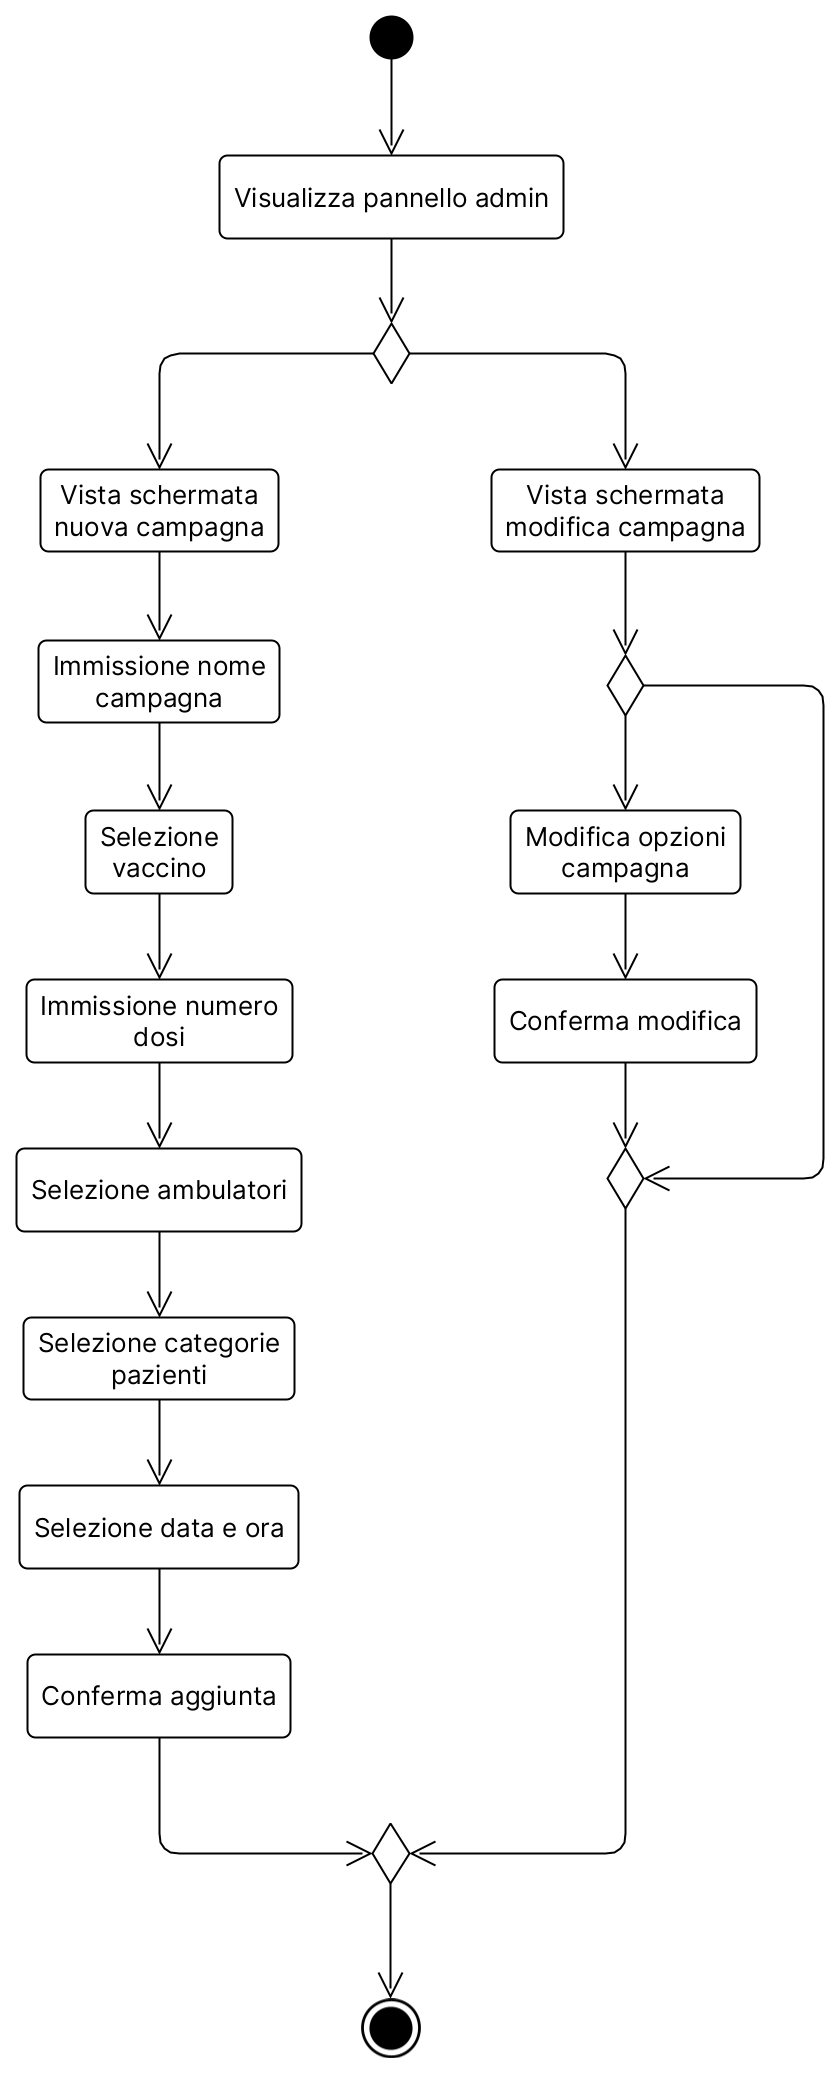
\includegraphics[scale=0.25]{ad_admin_create_yed.png}
    \end{figure}
\end{center}


\section{Sviluppo}

\subsection{Assunzioni e scelte progettuali}

La prima assunzione che è stata fatta sul progetto è che sia destinato ad una ASL che opera unicamente a livello regionale. Il sistema è stato dunque progettato per essere utilizzato in una singola regione italiana e dai suoi abitanti. Per questo motivo, si assume che venga fornito al software un file \texttt{Citizen.json} contenente un elenco di tutti i cittadini idonei ai vaccini della regione.

Si assume inoltre che venga effettuata una sola aggiunta, modifica o prenotazione della campagna alla volta per evitare inconsistenze di dati date dalla difficoltà di parallelizzare scritture su JSON.

\subsection{Progettazione ad alto livello e modelli architetturali}

Come pattern architetturale per questo progetto si è deciso di utilizzare MVC. La scelta di questo pattern si è rivelata la più sensata e ovvia per diverse ragioni: innanzitutto, la separazione netta e la modularità offerte da MVC permettono di migliorare enormemente la mantenibilità di questo sistema permettendo di effettuare modifiche future anche significative a basso costo. Per esempio, se in futuro si dovesse decidere di cambiare libreria per l'interfaccia grafica - magari a seguito del rilascio di un miglior sostituto a quella utilizzata o della deprecazione della stessa - sarebbe banale integrarla col progetto esistente: utilizzando l'architettura MVC il Model - ossia la parte che si occupa di gestire i dati e le operazioni associate non deve integrarsi direttamente con la GUI, ma solo esporre un'interfaccia che può essere facilmente implementata dalla vista Controller di qualsiasi frontend. Questa è una delle proprietà che rende questo pattern una scelta così gettonata per lo sviluppo di interfacce grafiche. Inoltre, poiché la libreria GUI utilizzata nel progetto - ossia JavaFX - utilizza internamente il pattern MVC e richiede un workflow basato su MVC, utilizzare questo pattern sull'intera codebase è risultata essere la migliore scelta per mantenere il codice semplice e coerente.

\begin{custlist}[,leftmargin=5.5em]
    \item[\textbf{Model}] gestisce i dati del sistema e si occupa di salvarli e ripristinarli dal database;
    \item[\textbf{View}] specifica la forma di rappresentazione delle informazioni del sistema all'utente, ossia l'interfaccia grafica;
    \item[\textbf{Controller}] fa da punto di raccordo tra il View e il Model: accetta l'input dell'utente e lo converte in comandi per Model e View.
\end{custlist}

Per chiarezza, le classi relative a questi tre componenti sono state organizzate in più pacchetti:

\begin{itemize}
    \item Le classi relative a \textbf{Model} si trovano nel pacchetto \texttt{it.vaxplan.backend}
    \item Le classi relative a \textbf{View} si trovano nel pacchetto \texttt{it.vaxplan.frontend}
    \item Le classi relative a \textbf{Controller} si trovano nel pacchetto \texttt{it.vaxplan.frontend.controller}
\end{itemize}


\subsection{Class diagram}

\begin{center}
    \begin{figure}
        \centering
        \caption{Digramma delle classi della vista Model}
        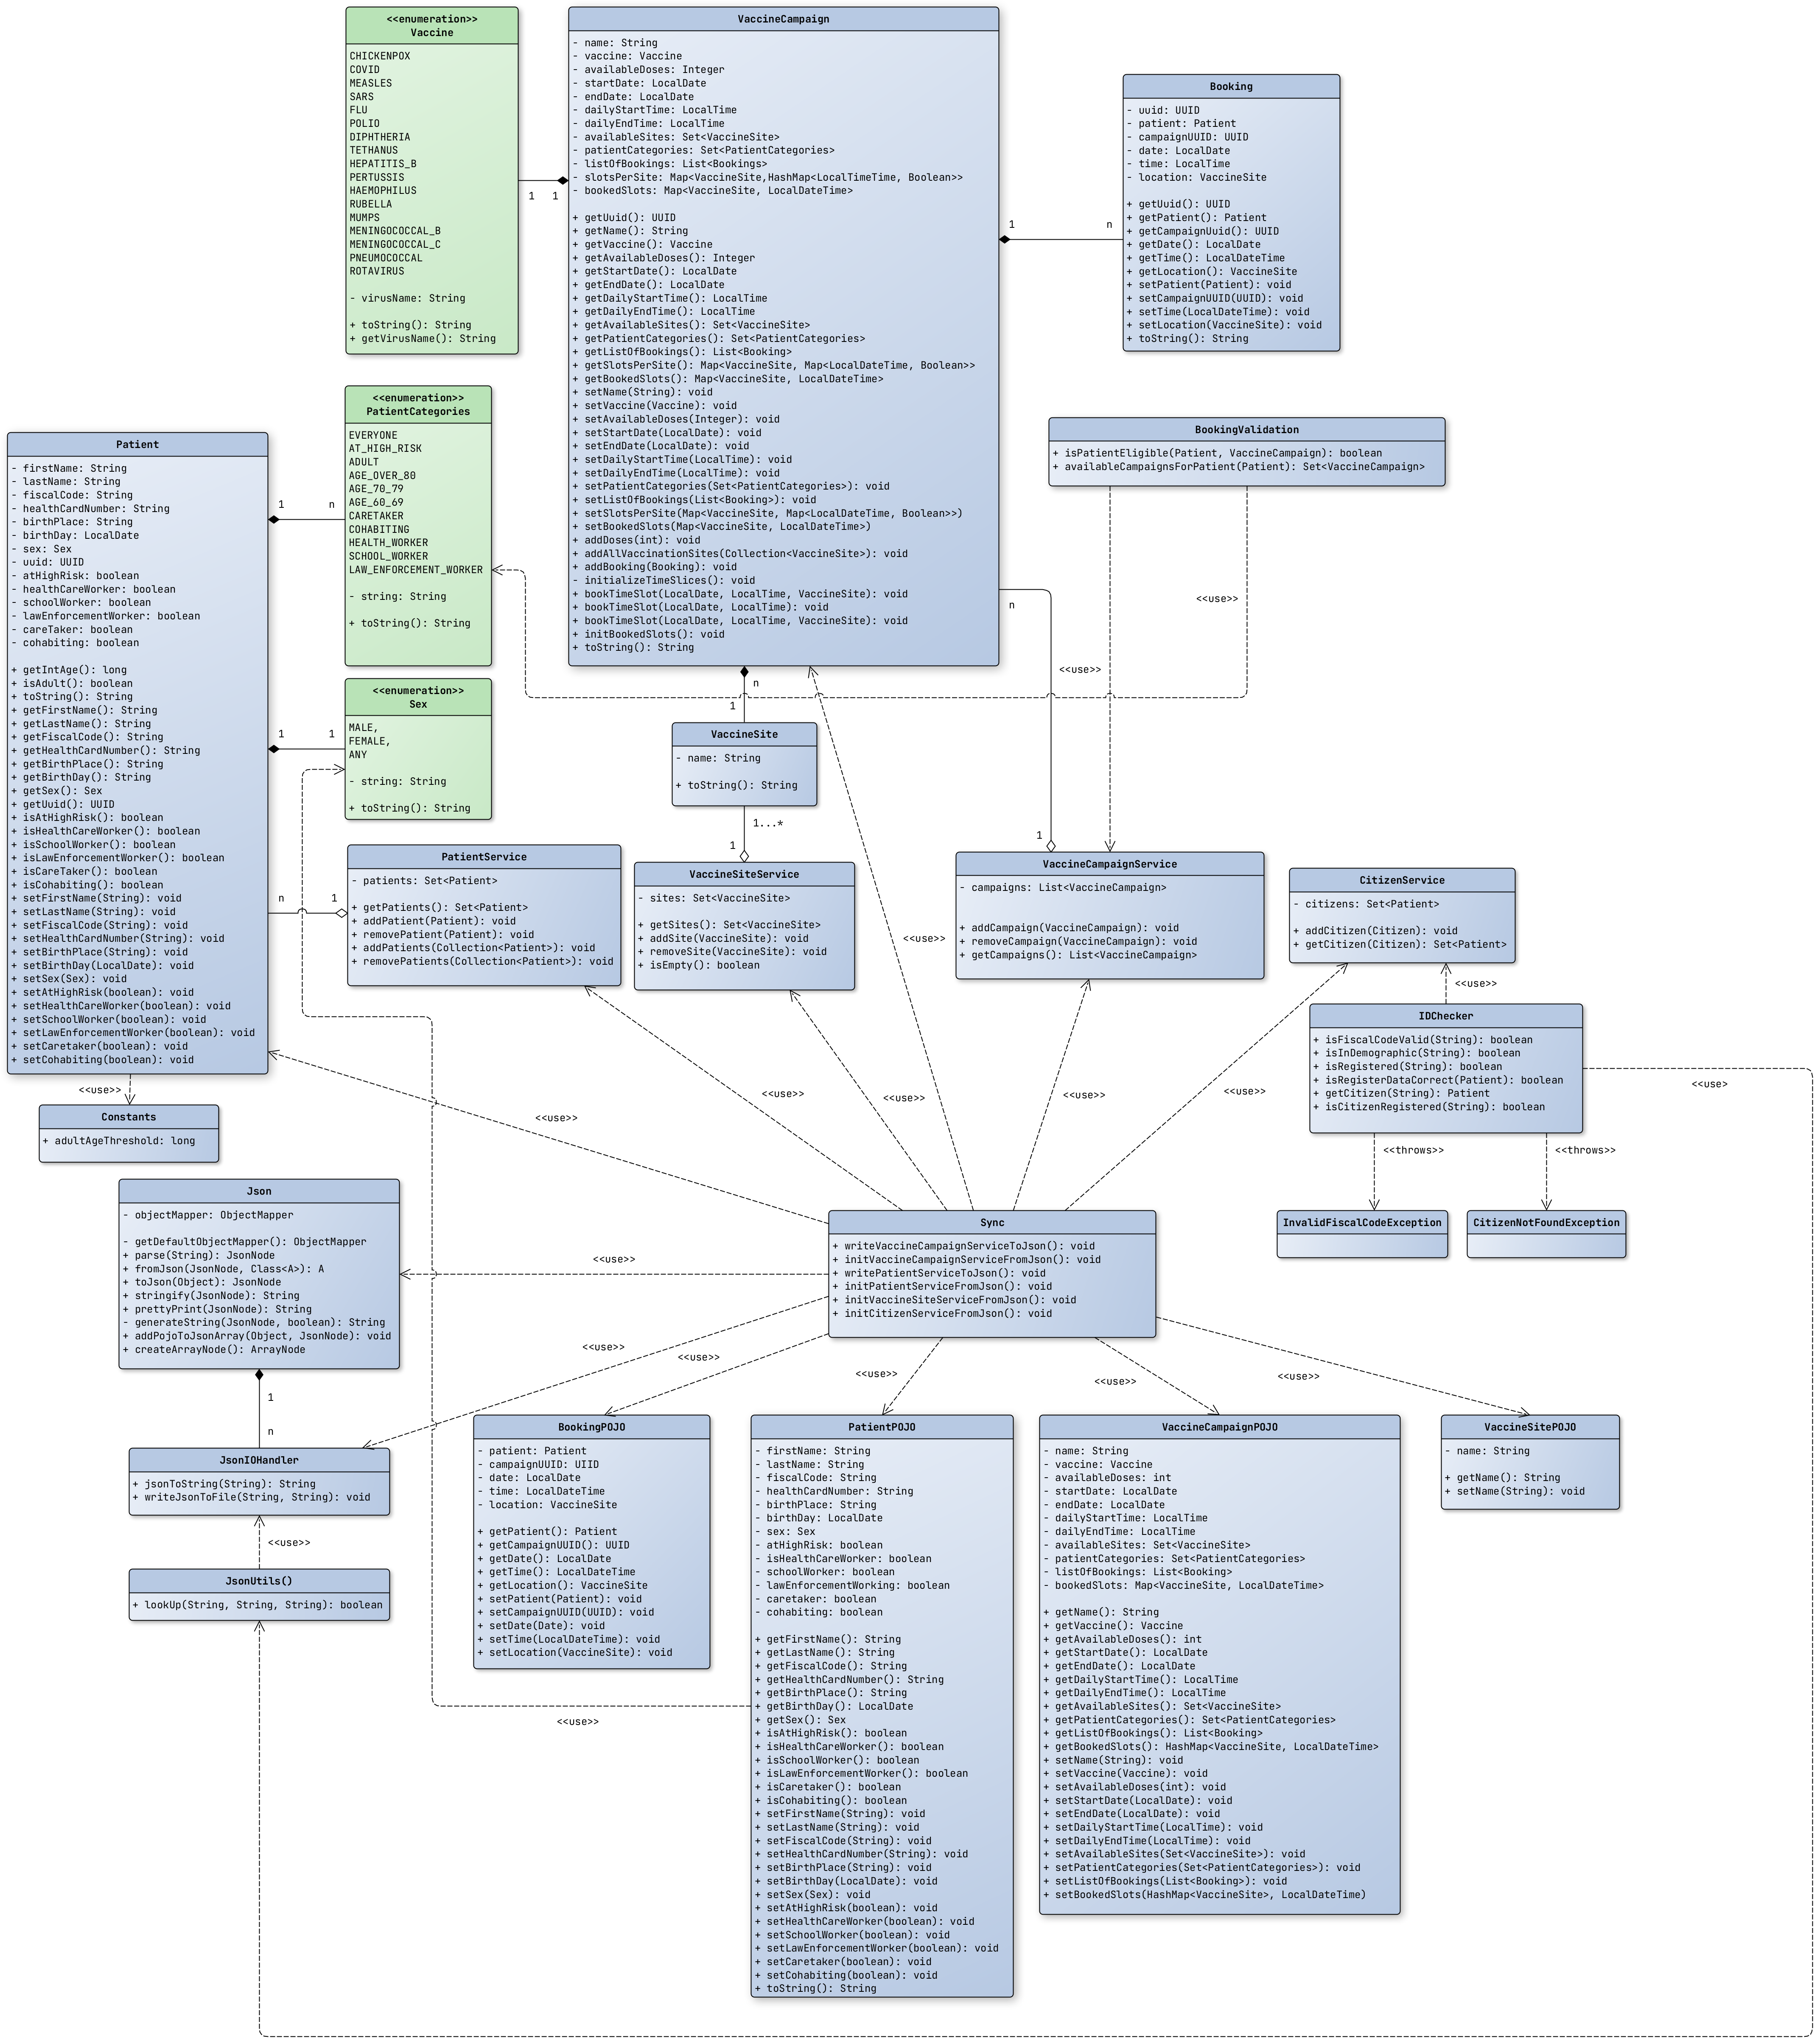
\includegraphics[scale=0.10]{class_diagram_model.png}
    \end{figure}
\end{center}

\begin{center}
    \begin{figure}
        \centering
        \caption{Digramma delle classi della vista View e Controller}
        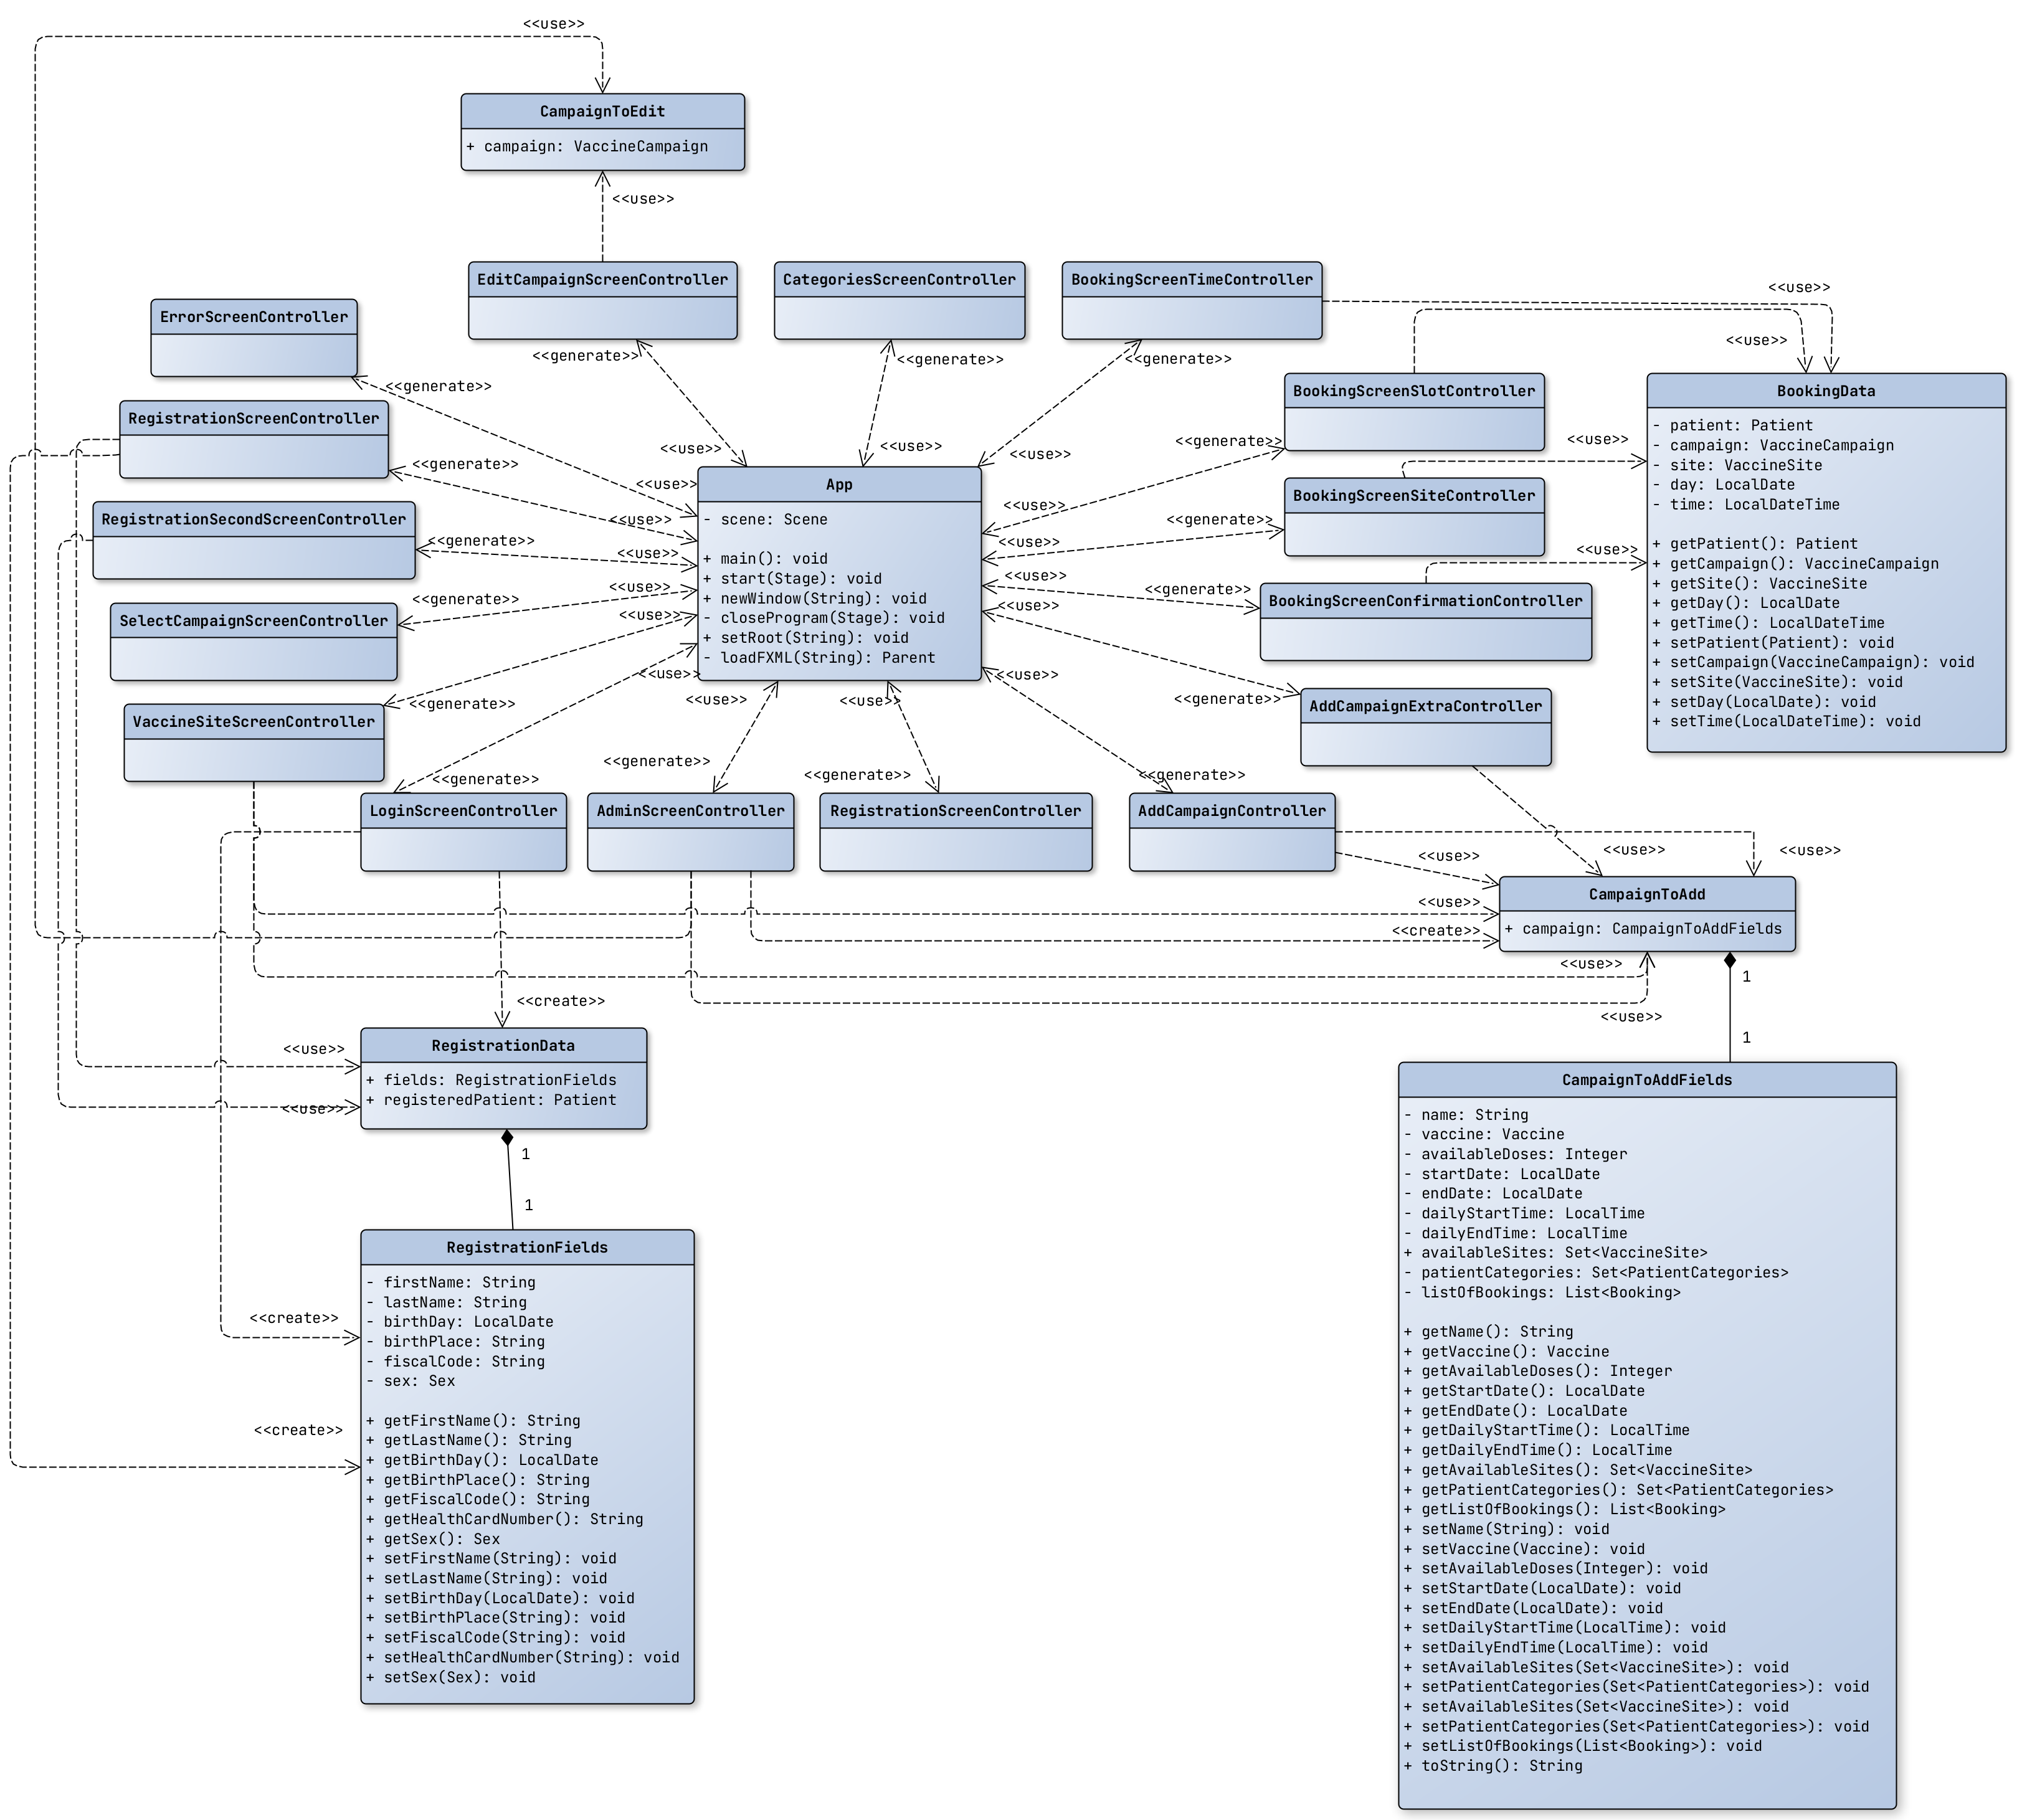
\includegraphics[scale=0.10]{class_diagram_view_controller.png}
    \end{figure}
\end{center}

Per quanto riguarda il Class Diagram corrispondente alla vista View e Controller, sono doverose alcune precisazioni.

In primis, le classi del Controller sono state istanziate nella sintassi UML come classi vuote: contengono infatti molti campi e metodi che sono utili \textit{esclusivamente} per l'implementazione a basso livello della GUI e avrebbero aggiunto eccessiva complessità al diagramma, al punto da pregiudicarne la stessa utilità.

In secundis, si noti come le classi Controller sono connesse alla classe \texttt{App} con una relazione di dipendenza con stereotipo \texttt{<<generate>>} dalla classe \texttt{App} alla classe Controller, e come non ci sia nessuna relazione tra i controller. Questo dipende dall'implementazione adottata da JavaFX quando si sceglie di definire l'interfaccia grafica utilizzando i file FXML, una tecnica di sviluppo più nuova che consente di velocizzare notevolmente lo sviluppo dell'interfaccia grafica. La classe \texttt{App} è la classe dove viene inizializzato lo \textit{stage} di JavaFX, in cui viene caricata una \textit{scena}, oggetto i cui metodi dovranno essere istanziati per caricare una nuova schermata nella finestra esistente. Questo caricamento viene fatto con il metodo \texttt{setRoot(String fxml)} della classe \texttt{App}, in quanto deve chiamare un metodo associato alla scene per caricare il file FXML il cui nome riceve in input dalla cartella resources.

Ogni file FXML contiene un attributo \texttt{fx:controller} che identifica la classe Controller associata a quella vista della GUI da inizializzare. Pertanto, la classe \texttt{App}, caricando un file FXML sulla \texttt{scene} principale, istanzia anche la classe definita nel suo \texttt{fx:controller}.

Sarebbe certamente stato possibile mettere in relazione i Controller con i propri file FXML associati nel diagramma avendo la cura di annotarle questi ultimi con stereotipo \texttt{<<artifact>>}, ma, una volta fatto questo, si è deciso di ometterli per evitare di sovrappopolare il diagramma al punto da pregiudicarne la leggibilità eccessivamente.

Si noti che esiste inoltre una relazione dalle classi Controller verso \texttt{App} con stereotipo \texttt{<<use>>}. Questo è giustificato dal fatto che, quando da un Controller associato ad una vista si desidera cambiare vista nella schermata corrente o creare una nuova schermata con una nuova vista al suo interno, bisogna utilizzare metodi della classe \texttt{App} per portare a termine l'operazione, non c'è nessuna relazione diretta tra il Controller della vista a che passa alla vista b e il Controller della vista b la cui visualizzazione segue alla vista a.

\subsection{Sequence diagrams}

\begin{center}
    \begin{figure}[H]
        \centering
        \caption{Sequence diagram "WelcomeScreenSequence" associato alla prima schermata visualizzata}
        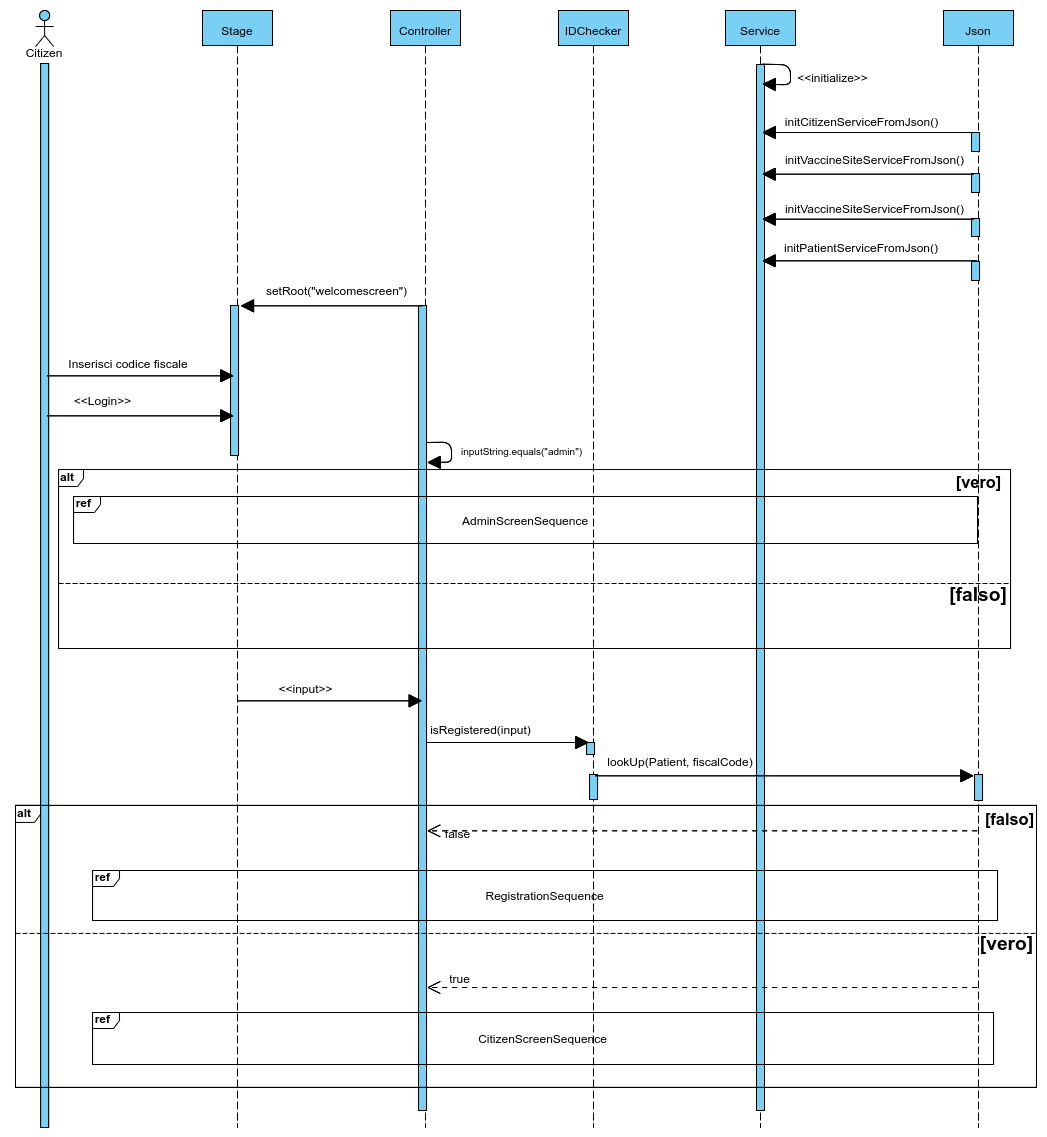
\includegraphics[scale=0.75]{WelcomeScreenSequence.png}
    \end{figure}
\end{center}

\begin{center}
    \begin{figure}[H]
        \centering
        \caption{Sequence diagram "RegistrationSequence" associato alla registrazione di un utente}
        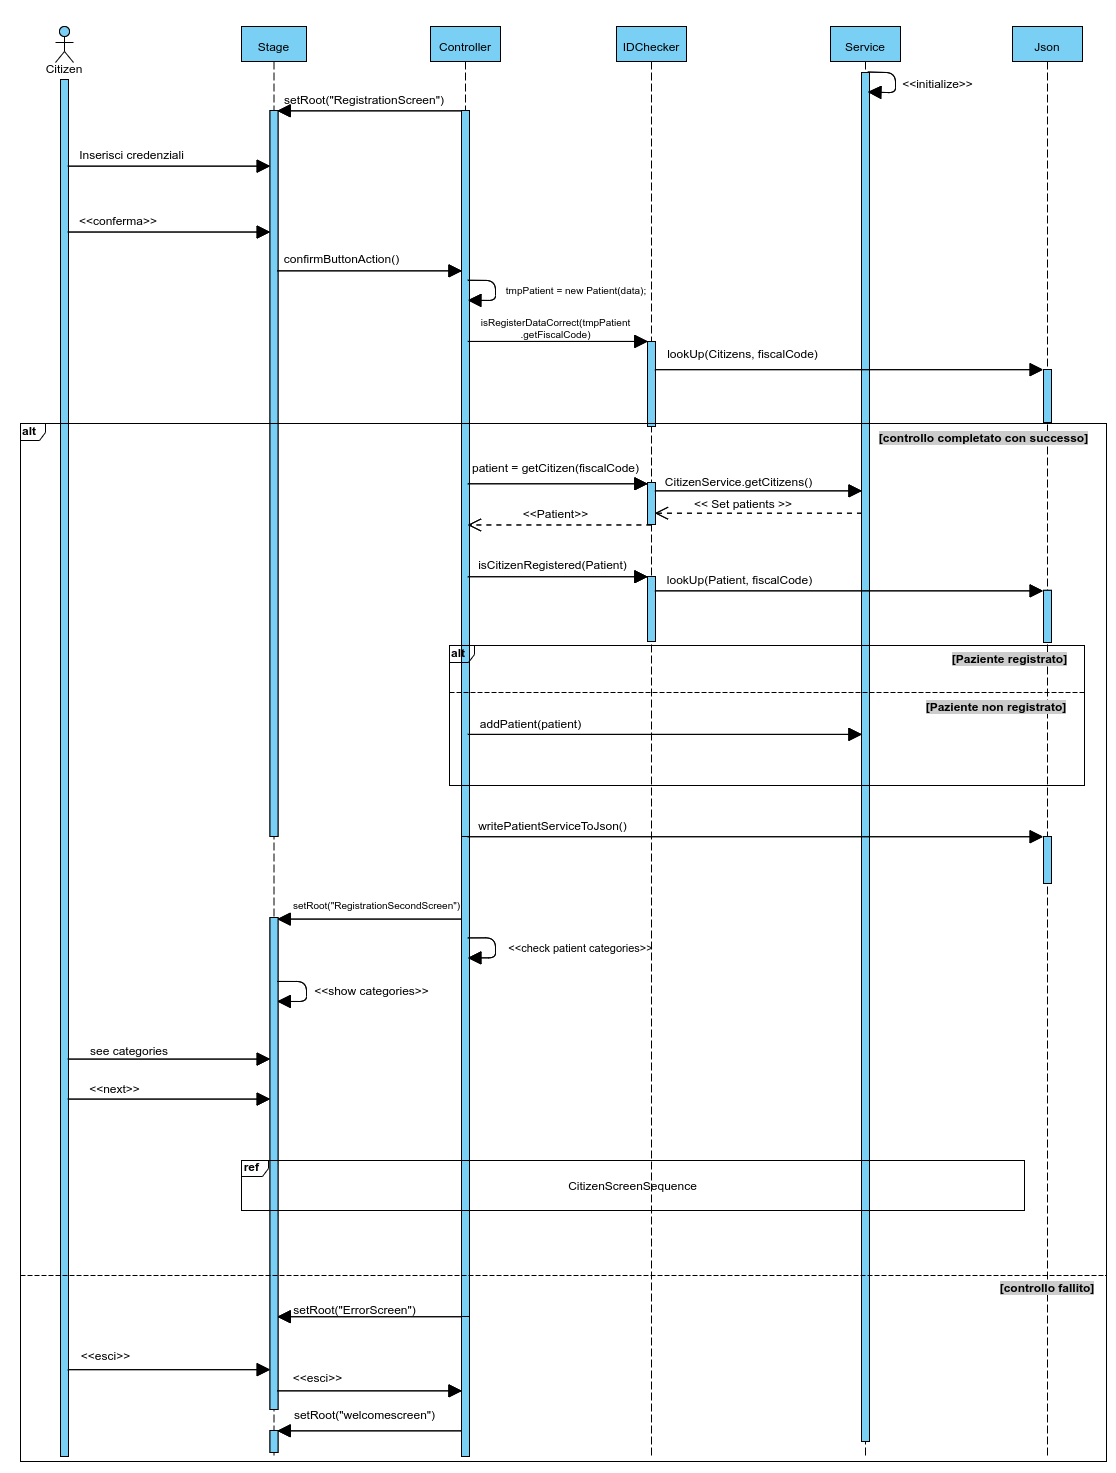
\includegraphics[scale=0.75]{RegistrationSequence.png}
    \end{figure}
\end{center}

\begin{center}
    \begin{figure}[H]
        \centering
        \caption{Sequence diagram "CitizenScreenSequence" associato alla registrazione di un appuntamento}
        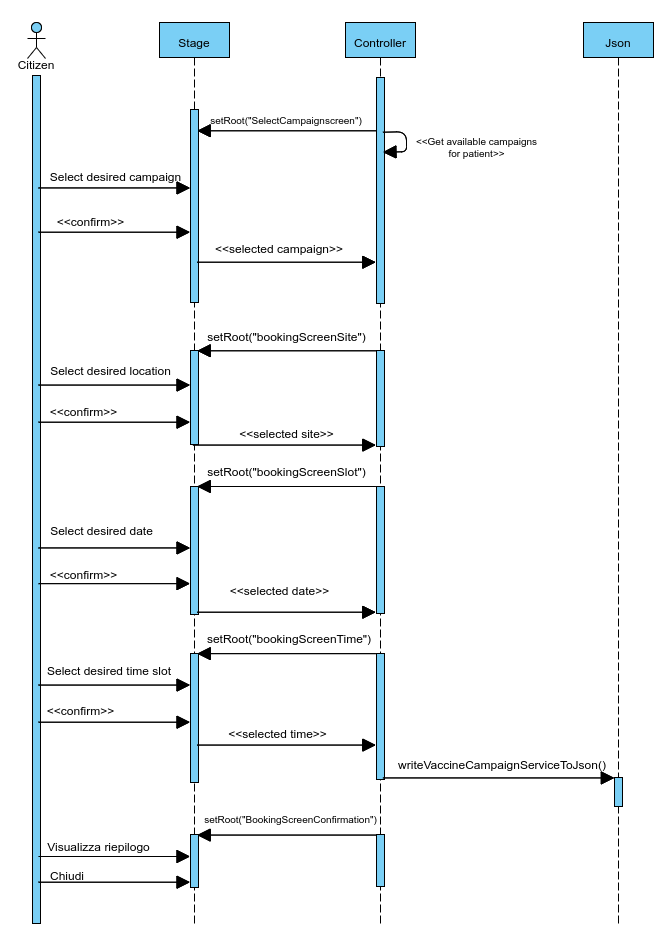
\includegraphics{BookingSequence.png}
    \end{figure}
\end{center}

\begin{center}
    \begin{figure}[H]
        \centering
        \caption{Sequence diagram "AdminScreenService" associato alla schermata admin}
        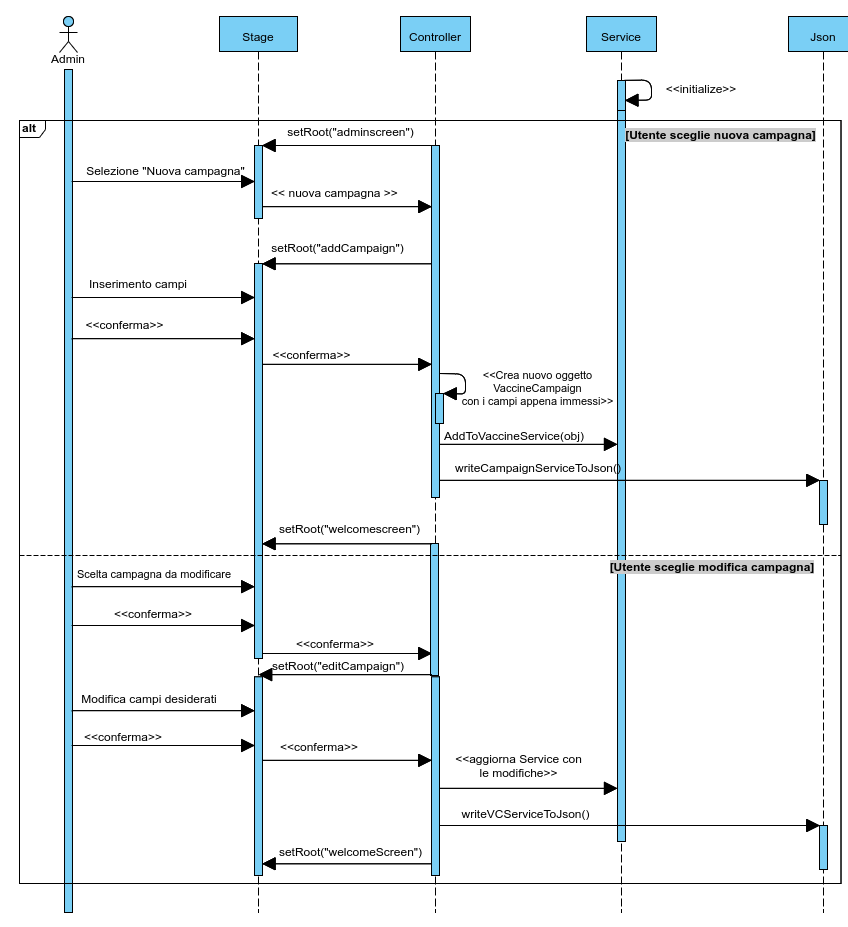
\includegraphics{AdminScreenSequence.png}
    \end{figure}
\end{center}

\begin{center}
    \begin{figure}[H]
        \centering
        \caption{Sequence diagram "InitServiceFromJsonSequence" associato all'inizlalizzazione dei Service dai file JSON}
        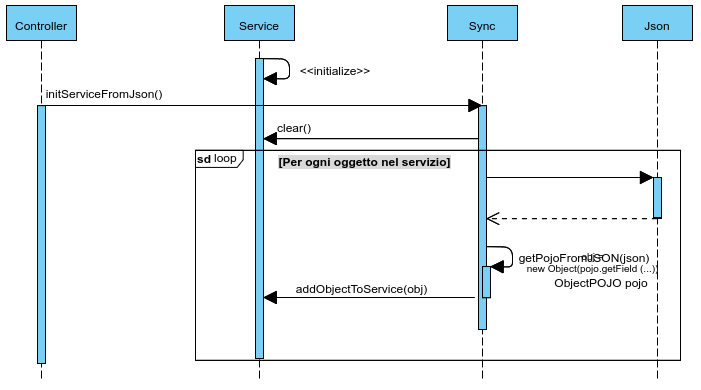
\includegraphics{InitServiceFromJsonSequence.png}
    \end{figure}
\end{center}

\begin{center}
    \begin{figure}[H]
        \centering
        \caption{Sequence diagram "WriteServiceToJsonSequence" associato alla scrittura dei Service sui file JSON}
        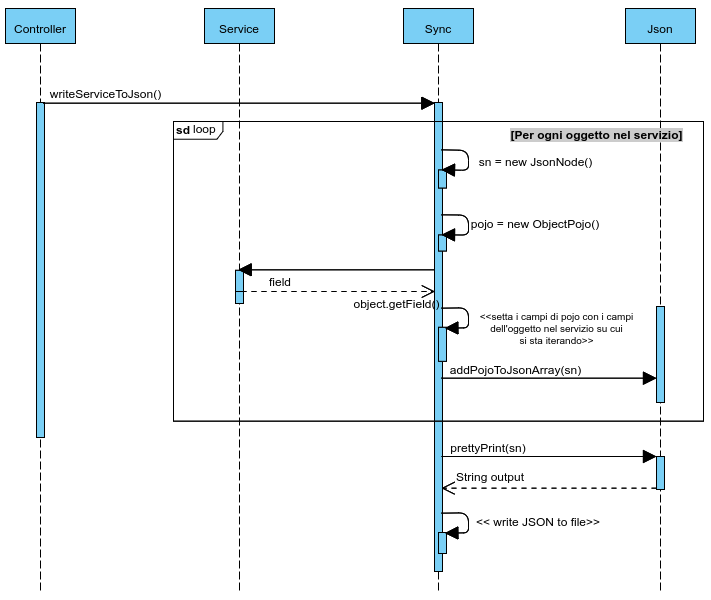
\includegraphics{WriteServiceToJsonSequence.png}
    \end{figure}
\end{center}

\newpage


\subsection{Design pattern}

Durante la fase di codifica del progetto sono stati impiegati i seguenti design pattern:

\begin{itemize}
    \item \textbf{Iterator Pattern}: Il pattern Iterator è utilizzato internamente da linguaggio Java e dalla sua libreria standard, pertanto è stato implicitamente utilizzato. Un chiaro esempio di utilizzo di questo pattern è trovabile nei metodi della classe \texttt{Sync} che vengono utilizzati per inizializzare i \texttt{Service} a partire dai file JSON: quest'ultimo viene parsato e convertito in un oggetto \texttt{JsonNode}, il quale espone un \texttt{Iterator} per accedere in maniera iterativa a tutti gli oggetti che contiene ed effettuarci operazioni - nel caso della classe \texttt{Sync}, convertirli in oggetti che possano essere aggiunti ai relativi \texttt{Service}.
    \item \textbf{Singleton Pattern}: È stato utilizzato occasionalmente il pattern Singleton per incapsulare oggetti con il compito di condividere informazioni tra più parti del prototipo, come in \texttt{RegistrationData} che istanzia un oggetto di tipo \texttt{RegistrationFields}, o similmente le classi \texttt{CampaignToEdit} e \texttt{CampaignToAdd}.
    \item \textbf{DAO Pattern (Data Access Object)}: Il codice che si occupa della (de)serializzazione dei JSON e dell'importazione dei dati da essi estratti nei \texttt{Service} che vengono utilizzati dalle varie classi del prototipo per gestire i dati seguono il design pattern DAO. La libreria Jackson Databind permette infatti di istanziare un oggetto \texttt{ObjectMapper}, che viene utilizzato nella classe \texttt{Json}, che è responsabile sia di ottenere i dati necessari dai file JSON, sia di aggiornarli con i nuovi dati ogni qualvolta i dati contenuti nei \texttt{Service} vengono modificati. A ciascuna classe \texttt{Service} corrisponde un Value Object intermediario POJO, ossia un oggetto molto semplice che si limita a mantenere gli stessi campi della classe di cui il \texttt{Service} tiene una Collection e di fornire relativi getter e setter. Questi oggetti vengono utilizzati come intermediari nella deserializzazione e nella serializzazione dei JSON per passare dati tra l'\texttt{ObjectMapper} wrappato nella classe \texttt{Json} e il resto del prototipo.
    \item \textbf{Facade pattern}: Rimanendo sempre sul tema della (de)serializzazione dei JSON, la classe \texttt{Sync} che si utilizza per coordinare le interazioni tra JSON e Service si basa a sua volta su una classe facade \texttt{Json}, la quale si occupa di istanziare un oggetto \texttt{ObjectMapper} (fornito da Jackson Databind), configurarlo ed esporre svariati metodi con cui è più facile interagire per nascondere alle altre parti del prototipo l'implementazione delle operazioni di parsing, deserializzazione, serializzazione (semplice o pretty-printed) senza dover interagire direttamente con l'\texttt{ObjectMapper} in \texttt{Sync}. Questo ha consentito di lavorare su quest'ultima classe con molto più agio, riducendo al minimo la duplicazione del codice e soprattutto evitando di riempire il resto del progetto con codice non banale da interpretare.
\end{itemize}

\subsection{Organizzazione e pianificazione del processo di sviluppo}

Per organizzare lo sviluppo del presente sistema sono state utilizzate metodologie di sviluppo incrementale ibride tra diverse tecniche di sviluppo agile, particolarmente incentrato sulla tecnica Scrum.

La prima fase di creazione dell'elaborato è stata una fase di progettazione ad alto livello: una volta presa in esame la specifica fornita ne sono stati estratti i requisiti non funzionali, i quali sono stati presi come vincolo per giudicare tutte le successive decisioni che sono state prese. Successivamente, sono stati delineati i primi requisiti funzionali, utilizzati come base per le fasi successive di progettazione. Ad ogni modo, non avendo utilizzato una metodologia di sviluppo strettamente plan-driven, questa decisione iniziale è stata una prima bozza che ha subito numerose revisioni durante il processo di sviluppo incrementale.

Successivamente, una volta delineati gli obiettivi principali del progetto, sono state prese le decisioni architetturali ad alto livello propedeutiche per il primo sprint di sviluppo vero e proprio. Lo sviluppo è stato diviso in più sprint, ciascuno dei quali incentrato sullo sviluppo di una feature in particolare. Ciascuno sprint si è composto fondamentalmente di quattro fasi:

\begin{enumerate}
    \item Revisione e perfezionamento delle decisioni già prese in precedenza
    \item Prima stesura del codice
    \item Scrittura e validazione con Unit Test
    \item Opportuni fix e refactoring, se necessari
\end{enumerate}

Si noti inoltre che, tra una fase di sviluppo e l'altra, sono sempre stati eseguiti gli Unit Test per verificare che tutti i singoli componenti interagissero correttamente anche a seguito delle modifiche appena apportate.

Il project management è stato condotto con il supporto di una kanban board - nello specifico, la webapp "Trello" - per delinare in maniera tangibile quali task si dovessero sviluppare, in quale ordine, secondo quali dipendenze e prerequisiti. Il lavoro è stato organizzato in più colonne - una per area concettuale - che contengono i task principali, resi con delle card, alcune delle quali racchiudono una checklist per suddividere il compito in una serie di sottoproblemi più piccoli.

Durante la fase di scelta dello stack tecnologico da utilizzare si è deciso di prendere ispirazione dalla tecnica "Integration and Configuration". Sebbene non sia stato utilizzato un intero framework di terze parti, si è comunque deciso di utilizzare e configurare opportunamente svariate librerie "off-the-shelf" per alleggerire i tempi di sviluppo di alcuni task che sarebbero risultati tediosi da reimplementare partendo dalle librerie standard di Java. Questa scelta ha consentito di rendere il codice di gran lunga più mantenibile, modulare e performante, poiché le prestazioni delle librerie di terze parti scelte sono superiori a quelle che sarebbero state ottenute reimplementando le stesse funzionalità con algoritmi più naive.

Il version control della codebase è stato fatto utilizzando Git, configurato per tracciare una repository remota su GitHub. Si è scelto di utilizzare un workflow multi-branch per consentire di mantenere contemporanemanete più stati del codice a diversi livelli di maturità, nonché per visualizzare la differenza delle modifiche tra una fase di sviluppo e l'altra in maniera semplice.

Per via di complicazioni legate alla pandemia in corso, il presente progetto è stato realizzato interamente da remoto. Oltre a Trello, abbiamo utilizzato il software "Code With Me" di IntelliJ IDEA - l'IDE per cui abbiamo optato - che consente di abilitare tecniche di pair programming da remoto condividendo a più persone connesse via Internet la stessa sessione dell'IDE dell'host. Inoltre, è stata utilizzata una piattaforma di videoconferencing per tutte le fasi di discussione e sviluppo.

\subsection{Librerie di terze parti utilizzate}

Per questo progetto si è scelto di utilizzare il linguaggio di programmazione Java ed il suo stack di sviluppo. Per gestire le librerie di terze parti, si è scelto di utilizzare Maven.

Le librerie che sono state utilizzate sono le seguenti:

\begin{itemize}
    \item \textbf{JavaFX}: Un toolkit GUI per Java che segue il modello architetturale MVC e utilizza la sintassi FXML per markup
    \item \textbf{Lombok}: Libreria di supporto che permette di ridurre di molto il boilerplate nel codice. Per esempio, permette di evitare la scrittura esplicita di costruttori, getter e setter nella maggior parte dei casi.
    \item \textbf{Jackson Databind}: Libreria che facilita la serializzazione e deserializzazione di JSON, formato di file che abbiamo deciso di utilizzare per memorizzare in maniera permanente i dati.
    \item \textbf{JUnit 5}: Una delle più popolari librerie di Unit Test per Java.
\end{itemize}

\section{Testing e validazione}

Il testing costante del sistema è stato uno dei punti chiave di ogni sprint di sviluppo. Questa si è rivelata una strategia vincente: effettuare testing costante sul codice dopo ogni cambiamento permette infatti di scoprire nuovi bug sul nascere, permettendo di correre ai ripari quando questo si può ancora fare con fix banali.

Le attività di test si sono composte delle seguenti fasi:

\begin{itemize}
    \item Verifica di consistenza con le specifiche
    \item Verifica di consistenza con il progetto ad alto livello, eventuale modifica del codice o delle decisioni ad alto livello prese
    \item Esecuzione di diversi casi d'uso (GUI)
    \item Scrittura di Unit Test
    \item Esecuzione di Unit Test
    \item Eventuali bugfix
    \item Monitoring del processo con un system monitor per verificare che l'utilizzo di CPU e di memoria si mantenga normale per tutta l'esecuzione, nel tentativo di identificare immediatamente eventuali memory leak o altri gravi problemi di prestazioni
\end{itemize}

\subsection{Unit test}

La metodologia di testing più potente tra quelle impiegate è stata senz'altro l'Unit Testing con JUnit5.

Per ciascuna delle classi principali del Model è stata scritta una corrispondente classe di test, che è stata successivamente popolata con diversi Unit Test, alcuni volti a riprodurre sequenze di azioni comunemente incontrate nei casi d'uso previsti dal software, altri volti a testare il software con vari e particolari input per verificare la sua resilienza e robustezza. Questo ha permesso di produrre un codice robusto e accettabile, caratteristiche fondamentali per un software rivolto al settore ospedaliero.

L'utilizzo di Unit Test ha velocizzato notevolmente la fase di test, essendo l'esecuzione di un test molto più veloce che provare a riprodurre un determinato scenario manualmente, dall'interfaccia grafica.

Infine, è degno di nota che l'utilizzo degli Unit Test consente di sapere quanto tempo ogni test ha impiegato per completare, informazione molto utile per identificare eventuali anomalie. Questa caratteristica in particolare è stata immensamente utile per scoprire e rimediare a un overhead nella parte del codice che si occupa del parsing dei file JSON, risultando in un progetto più performante e ottimizzato.

Nello specifico, tra le casistiche controllate rientrano:

\begin{itemize}
    \item (De)serializzazione di oggetti JSON
    \item Scrittura su file degli oggetti JSON
    \item Lettura da file dagli oggetti JSON
    \item Validazione dei codici fiscali
\end{itemize}

\subsection{Test manuali degli sviluppatori}

Per quanto molto utili per la vista Model del software, gli Unit Test di JUnit5 non sono purtroppo adatti a verificare con precisione il corretto comportamento delle viste View e Control, vale a dire, quelle associate all'interfaccia grafica. Per questo motivo, sono stati eseguiti ad ogni sprint diversi test manuali sull'interfaccia grafica stessa. Alcuni dei test svolti sono:

\begin{itemize}
    \item \textbf{Verifica del corretto funzionamento dell'autenticazione}: È consentito autenticarsi al sistema solo a cittadini che vi sono stati registrati. Ai cittadini non registrati viene mostrata una schermata di registrazione in seguito al tentativo fallimentare di effettuare il login.
    \item \textbf{Verifica del corretto funzionamento della registrazione}: Poiché si ragiona sotto l'assunzione che la ASL che usufruirà del software opera solo a livello regionale, si permette solo ai cittadini registrati nel database demografico della regione provvisto di effettuare la registrazione. Se i dati anagrafici inseriti dall'utente non corrispondono ad una persona che si trova in questo record, non sarà permesso all'utente registrarsi al sistema. A registrazione avvenuta, le categorie di pazienti visualizzate devono corrispondere a ciò che è scritto sul JSON del database della regione nell'oggetto JSON corrispondente al cittadino appena registrato.
    \item \textbf{Aggiunta di una campagna vaccinale}: Una campagna vaccinale deve poter essere aggiunta solo se l'addetto ASL ha fornito tutti i campi necessari e se le date e ore di fine sono temporalmente future rispetto alle date e ore di inizio, la campagna deve essere leggibile, tutti i suoi campi devono corrispondere perfettamente con l'input in fase di creazione e deve essere scritta correttamente e per intero sul JSON associato.
    \item \textbf{Modifica di una campagna vaccinale}: Dopo la modifica, tutti i campi della campagna che sono stati modificati devono corrispondere al nuovo valore, così come la rappresentazione su JSON della campagna.
    \item \textbf{Esecuzione di più operazioni nella stessa sessione}: Portando a termine diverse delle operazioni precedenti nella stessa sessione il comportamento del software deve mantenersi prevedibile, senza causare crash o corruzione di dati. Inoltre, interrompere un caso d'uso interrompibile prima del completamento non deve modificare né i relativi dati in memoria né la loro rappresentazione su JSON. Queste modifiche devono essere apportate solo nel passo terminale dell'attività.
\end{itemize}

\subsection{Validazione del codice}

La correttezza del codice è stata validata principalmente con due strumenti: il checking integrato nell'IDE "IntelliJ IDEA" in primis, e \textbf{SonarLint} in secundis.

SonarLint è un'estensione per IDE che integra il controllo statico di \textit{correttezza} del codice integrato nell'IDE scelto con ulteriori check di \textit{qualità} e \textit{sicurezza}. SonarLint, oltre che notificare allo sviluppatore la presenza di codice scorretto, segnala anche eventuali cattive pratiche che possono dare luogo a problemi o falle di sicurezza in futuro. L'utilizzo di uno strumento del genere consente di mantenere alte mantenibilità, robustezza e accettabilità del codice semplificando la scrittura di un sistema robusto e scritto secondo le \textit{best practice} di Java.

Per esempio, seguendo i suggerimenti di SonarLint, tutte le classi utility (vale a dire, classi che contengono unicamente campi o metodi \texttt{static}) sono state dotate di un costruttore privato che nasconde quello di default e lancia una \texttt{IllegalArgumentException()} se si prova ad istanziare la classe. Grazie a questo accorgimento, uno sviluppatore nuovo al progetto che si trova a lavorare su una codebase esistente ha meno possibilità di commettere un errore banale dato dalla momentanea scarsa familiarità con il codice per via di accorgimenti come questo.

\subsection{Organizzazione della documentazione}

Il sistema è stato documentato utilizzando \textbf{JavaDoc}, un applicativo incluso nel JDK utile per generare automaticamente una documentazione del codice in HTML annotando metodi, classi o campi che si desidera documentare con una speciale notazione. Tutti i metodi principali sono stati accuratamente annotati seguendo gli standard di JavaDoc.

Oltre a permettere di generare una documentazione HTML del progetto, utilizzare JavaDoc ha consentito di servirsi dell'integrazione nell'IDE, che permette di consultare la JavaDoc di qualsiasi metodo facendo mouse over su di un utilizzo di esso. L'utilizzo della funzionalità di consultazione rapida della JavaDoc integrato in IntelliJ IDEA ha consentito di velocizzare notevolmente i tempi in fase di sviluppo.

Inoltre, documentare bene un codice è imperativo per garantire la mantenibilità di un progetto. Una codebase leggibile e ben documentata sarà infatti relativamente facile da utilizzare da un nuovo sviluppatore in futuro, caratteristica auspicabile in un software enterprise.

Per ragioni di consistenza, pur essendo il progetto rivolto al sistema ospedaliero italiano, tutta la documentazione è stata scritta in lingua inglese, così come i nomi di classi, campi e metodi.

\subsection{Test del prodotto finale su utenti}

Al termine della fase di sviluppo, alcune persone completamente esterne allo sviluppo sono state sottoposte ad un processo di test: hanno dovuto svolgere determinate mansioni con il prototipo finito con minima guida. I soggetti di test sono stati in grado di portare a compimento tutti i casi d'uso principali senza problemi, aiutando tuttavia a scoprire alcuni bug ancora presenti nel software che sono sfuggiti alla fase di test da parte degli sviluppatori.

\newpage










\end{document}
